\section{Runtime Enforcement}
\label{sec:av_enforcement}

%Runtime enforcement techniques are lightweight and do not require a formal model of the system since only the executions of the system are considered, hence, it is very much suitable for monitoring and enforcing critical properties of safety-critical systems.

Using formal runtime monitoring approaches and tools, verification/enforcement monitors (enforcers) can be synthesized from the formal requirements of desired policies, which can be integrated with the system (as shown in Figure \ref{fig:RE}). The enforcer is fed with the current execution of the system. It verifies the current execution with respect to the desired policies and enforces (corrects) the current execution when dealing with the enforcement of the desired safety policies at runtime. 
\begin{figure}[H]
    \centering
    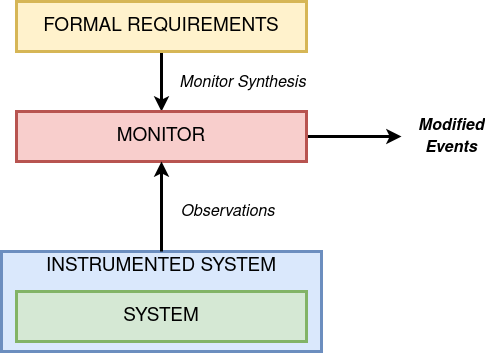
\includegraphics[width=0.6\linewidth]{sections/av/fig/RE.png}
    \caption{An overview of runtime enforcement process}
    \label{fig:RE}
\end{figure}


\subsection{Enforcer Synthesis} 
In our work, we use the enforcer synthesis tools that are based on the approaches proposed in \cite{10.1109/TII.2019.2945520} that are suitable for safety-critical and cyber-physical systems. The framework in \cite{10.1109/TII.2019.2945520} supports RE monitor synthesis for timed
policies. Valued Discrete Timed
Automata (VDTA) is used for the formal specification of policies, where valued signals, internal variables, and complex guard conditions are supported, ensuring compatibility with real-world CPS and industrial systems and enforcement monitors are synthesized from these VDTA to enforce a set of desired policies.\\

\noindent \textit{Prelimineries to RE.} A (finite) word is a finite sequence of elements of finite alphabet $ \Sigma $. 
The length of $ w $ is the number of elements in $ w $ and is denoted as $ | w | $.  
%The empty word over $ \Sigma $ is denoted by $ \epsilon $. 
The sets of all words are denoted by $ \Sigma^{\ast} $. 
A language (property) over $ \Sigma $ is any subset of $ \Sigma^{\ast} $ and is denoted by $\varphi$. 

Let $\mathbb{R}$ denote the set of real numbers. $M:\mathbb{R}^n \rightarrow \mathbb{R}^m$ is a function which takes as input a vector of $n$ real valued numbers and gives as output a vector of $m$ real valued numbers. This function represents an ANN model. \\


\noindent \textit{Enforcer for $\varphi$.} An enforcer (from \cite{10.1109/TII.2019.2945520}) for a property $\varphi$  is a function $E_{\varphi} : \Sigma^{\ast} \rightarrow \Sigma^{\ast}$ that takes as input a word $\Sigma^{\ast} $ and outputs a word that satisfies $\varphi$ or can be extended to satisfy $\varphi$ in the future. It can only edit an input event when necessary, and it can not block, delay or suppress events.\\

Some constraints are required on how an enforcer transforms words. These constraints describe the expected behaviour of an enforcer and are recalled below (Def. from \cite{}).
\begin{definition}
    Given property $\varphi$, an enforcer for $\varphi$ satisfies the following constraints:
        \begin{flushleft}
            \textbf{Soundness:}
        \end{flushleft}
		% \vspace{-1em}
        \begin{equation*}
            \label{eq:snd}
              \forall \sigma \in \Sigma^{\ast}, \exists \sigma_{extn} \in \Sigma^{\ast} : E_{\varphi} (\sigma) \cdot \sigma_{extn} \models \varphi
        \end{equation*}
        
        \begin{flushleft}
            \textbf{Monotonicity:}
        \end{flushleft}
		% \vspace{-1em}
        \begin{equation*}
            \label{eq:mo}
              \forall \sigma, \sigma_{extn} \in \Sigma^{\ast}: \sigma \preccurlyeq \sigma_{extn} \implies E_{\varphi} (\sigma) \preccurlyeq E_{\varphi} (\sigma_{extn}).
        \end{equation*}	

        \begin{flushleft}
            \textbf{Transparency:}
        \end{flushleft}
		% \vspace{-1em}
        \begin{equation*}
            \label{eq:tr}
              \forall \sigma, a, \sigma_{extn} \in \Sigma^{\ast} : E_{\varphi} (\sigma) \cdot a \cdot \sigma_{extn} \models \varphi \implies E_{\varphi} (\sigma \cdot a) = E_{\varphi} (\sigma) \cdot a.
        \end{equation*}	
        \label{constraints1}
\end{definition}
\textit{Soundness} means that for any input word, the output of the enforcer can be extended to a sequence that satisfies $\varphi$. \textit{Monotonicity} means that the output is a continuously growing word: the output of the enforcer for an extended input word $\sigma_{extn}$ of an input word $\sigma$, extends the output produced by the enforcer for $\sigma$. %i.e., for a given input word, what is output can only be changed by appending new events. 
\textit{Transparency} 
\footnote{\cite{1} presents a bidirectional enforcer, whereas our approach focuses on a unidirectional enforcer. Our enforcer corrects inputs from the system in a single direction and is synthesized using the monitor synthesis approach outlined in \cite{1} only. Consequently, the transparency constraints defined in Def. \ref{constraints1} of our work are slightly modified compared to those in Def. 2 of \cite{1}.} 
means that the enforcer will not unnecessarily edit any event i.e., for any given input sequence $\sigma$ and any input event $a$, if the output of the enforcer for $\sigma$ (i.e., $E_{\varphi} (\sigma)$) followed by the input event $a$ has a extension $\sigma_{extn}$ such
that $E_{\varphi} (\sigma) \cdot a \cdot \sigma_{extn}$ satisfies the property $\varphi$, then the output that the enforcer produces for input
$\sigma \cdot a$ will be $E_{\varphi} (\sigma) \cdot a$.
    

Some other constraints are required, specifically to respect synchronous execution in reactive systems, such as \textit{instantaneity} and is recalled below (Def. from \cite{}). 
\begin{definition}
    Given property $\varphi$, an enforcer for $\varphi$ satisfies the following constraint:
        \begin{flushleft}
            \textbf{Instantaneity:}
        \end{flushleft}
        \vspace{-1em}
        \begin{equation*}
            \label{eq:Ins}            
              \forall \sigma \in \Sigma^{\ast}: | \sigma | ~=~ | E_{\varphi} (\sigma )|
        \end{equation*}
        \label{constraints2}
\end{definition}

\textit{Instantaneity} means that for any given input sequence, the length of the output sequence of the enforcer should be the same as the input sequence. This means that the enforcer cannot delay, insert and suppress events. Whenever the enforcer receives a new input event, it must react instantaneously and produce an output event immediately. This requirement is essential for the enforcement of CPSs, which are reactive in nature. \\


\noindent \textit{Edit Functions.} Given property $\varphi$, we introduce $edit_{\varphi}$, which the enforcer uses for
editing input events (whenever necessary), to satisfy property $\varphi$. This definition is an adapted version of the edit function presented in Sect. 2.2 of \cite{}. The adaptation eliminates bidirectionality, resulting in a purely unidirectional enforcer.
\begin{definition}[Edit function]
    Given an input word $\sigma \in \Sigma^{\ast}$ and an input event $x \in \Sigma$, $edit_{\varphi}(\sigma, x)$ is the set of events $x' \in \Sigma$ such that the word obtained by extending $\sigma$ with $x'$ can be extended to a sequence that satisfies the property $\varphi$ (i.e., $\exists \sigma_{extn} \in  \Sigma^{\ast}$ such that $\sigma \cdot x' \cdot \sigma_{extn} \models \varphi$). Formally,
    \begin{align*}
        edit_{\varphi}(\sigma, x) = \{x' \in \Sigma:~ \exists \sigma_{extn} \in  \Sigma^{\ast}, \sigma \cdot x' \cdot \sigma_{extn} \models \varphi\}
    \end{align*}
\end{definition}
Two proposed methods for editing non-accepting input values are given in \cite{}. These are either a random edit, where a random but accepting value would be chosen from a list of accepting values; or a minimum distance edit, where an accepting value would be chosen with minimum binary distance compared to the current
non-accepting value.

\begin{remark}[Soundness, Monotonicity, Transparency and Instantaneity]
    It has been proved that the enforcer synthesized using the approach outlined in \cite{} satisfies soundness, monotonicity, transparency and instantaneity constraints given in Def \ref{} and \ref{}.
\end{remark}

Since our system is composed of (ML) models connected sequentially or in parallel with an enforcer connected after the entire system, we define properties, such as \textit{inter-model consistency} and \textit{robustness}. %, which were not guaranteed without enforcers. 

%The intuition behind \textit{error containment} is that, in a compositional model, errors from one model can propagate to subsequent models, potentially compounding inaccuracies. With the \textit{sound} enforcers placed after each model \sout{in the sequence}, the system ensures that the output of each stage satisfies the local property $\varphi$. This reduces error propagation and ensures correctness at each stage.

The concept of \textit{inter-model consistency} arises from the observation that, in a decomposed ML system, multiple smaller models $M_1,\cdots M_k$ are interconnected. The output of one model often serves as the input to the next, forming a sequence of dependencies. The enforcer operates after the entire system, ensuring that the final output satisfies a global property $\varphi$. The intuition behind \textit{inter-model consistency} is that the relationships and dependencies between sub-models $M_1,\cdots M_k$, are conserved by the enforcer $E_{\varphi}$ even after corrections, i.e., their intended role and do not contradict each other after correction.



The concept of \textit{robustness} arises from the observation that an ML model may fail to handle adversarial or unexpected inputs, potentially resulting in unsafe or unreliable behavior. By placing enforcer after the (decomposed) model, the system ensures operation within predefined bounds, even in scenarios that were not covered during training. In essence, an enforcer acts as a runtime safeguard in managing edge cases and adversarial inputs effectively.

\begin{definition}
    Given $n$ decomposed models $M_1, \cdots M_n$, given input vector $x_1, \cdots, x_n$ to each model and given an enforcer $E_{\varphi}$ for property $\varphi$, placed after the entire decomposed model, whose final output is obtained by $E^{out}$. %Let $M_i(x_i)$ denote the output of the model $M_i$ for input $x_i$ which is fed as an input to enforcer $E_i$ and let $y_{i+1}=E_i(M_i(x_i))$ denote the output of the enforcer $E_i$. 
    The system satisfies the following constraint:
    % \begin{flushleft}
    %         \textbf{Error Containment: \saumya{not correct}}
    % \end{flushleft}
    % \begin{equation*}
    %     \label{eq:ep}            
    %     \forall i \in (1,n): E_{\varphi_i}(M_i(x_i))=x_{i+1} \implies \exists \sigma_{i}' : ~x_{i+1} \cdot \sigma_{i}' \models \varphi_i
    % \end{equation*}
    \begin{flushleft}
            \textbf{Inter-model consistency:}
    \end{flushleft}
    \begin{equation*}
        \label{eq:ro}            
        E^{out} \models \varphi \implies \Bigl( \forall M_j: M_i \rightarrow M_j %M_i, M_j \in \{M_1,\cdots M_k\} 
        \implies M_j({M_i}^{corr}({x_i}^{corr})) \sim M_j(M_i(x_i)) \Bigr)
    \end{equation*}
    \begin{flushleft}
            \textbf{Robustness:}
    \end{flushleft}
    \begin{equation*}
        \label{eq:ro}            
        % \forall \sigma_{adv_i} \in \Sigma^{\ast} \implies E_{\varphi_i}(M_i(\sigma_{adv_i})) \models \varphi_i
         \forall M_i \in \{M_1, \cdots, M_n\}, \forall \sigma_{adv} \in \Sigma^{\ast} 
         \Bigl(M_i(\sigma_{adv})  \implies E^{out} \models \varphi \Bigr)
    \end{equation*}
    \label{constraints3}
\end{definition}

%\textit{Error containment} means that there exists a potential extension $\sigma_i'$ of the output sequence $x_{i+1}$ satisfying property $\varphi_i$ at each stage. This means that for the composition of enforcers, it is ensured that each stage validates and corrects the output before it is passed to the next stage. Thus, the error propagation is reduced.

\textit{Inter-model consistency} expresses that if $M_i$ is corrected by the enforcer to produce ${M_i}^{corr}({x_i}^{corr})$, given any model $M_j$ that depends on $M_i$'s output must still behave compatibly with how it would have behaved with the original, uncorrected output $M_i(x_i)$ provided the final enforced output $E^{out}$ satisfies property $\varphi$. It means that the relationships and dependencies between sub-models $M_1,\cdots M_k$, are conserved by the enforcer even after corrections. Here, $\sim$ denotes compatibility, i.e., $M_j({M_i}^{corr}({x_i}^{corr})) \sim M_j(M_i(x_i))$ if they belong to same valid input space.

%\textit{Robustness} means that for any adversarial input $\sigma_{adv_i}$ the enforcer guarantees property satisfaction.
\textit{Robustness} means that for every model $M_i$ and every adversarial input $\sigma_{adv}$, the enforcer ensures that even if $M_i$ produces an incorrect or unsafe result due to $\sigma_{adv}$, the final output of the enforcer $E^{out}$ will satisfy the required property $\varphi$. In simpler terms, no matter how an adversarial input impacts the models, the enforcer ensures the system adheres to the property.

\begin{proposition}[Inter-model consistency, Robustness]
    Given a property $\varphi$, its enforcer $E_{\varphi}$ satisfies Inter-model consistency and Robustness constraints as per Def. \ref{constraints3}.
    \label{propo1}
\end{proposition}
